%
%  == Collective paper on MORSE for HRI ==
%
%
% Editing of the article moves to GIT (Sharelatex does not expose the change history unless you
% pay for it, so it's difficult to track changes and merge them with GIT).
%
% The repo is here:  https://github.com/morse-simulator/publication-iros2014-hri
%
%
% The idea is: each of you present (in one section) its project, 
% putting an emphasis on:
%   1- why simulation is useful/needed for your use-case
%   2- is it satisfactory or not
%   3- what is good and could be useful to other researcher
%   4- what is missing both at the technical level (things that could be added 
%      to MORSE) and at a more fundamental level (things where simulation do 
%      not fit)
%
% It would be great to have one nice screenshot per project.
%
% Then, Severin and Florian write a synthesis in the conclusion.
%
% Severin will also write a short introduction + presentation of MORSE for HRI
%


\documentclass[conference]{IEEEtran}

% UTF8 support
\usepackage[utf8x]{inputenc}
\usepackage[T1]{fontenc}
\usepackage{url}
\usepackage{graphicx}
\usepackage{float}

\usepackage[draft]{fixme}
\usepackage{todonotes}

\graphicspath{{figs/}}
\newcommand{\eg}{{\textit{e.g.~}}}
\newcommand{\etal}{{\textit{et al.~}}}
\newcommand{\ie}{{\textit{i.e.~}}}

\begin{document}

\title{Simulation and HRI: Recent Perspectives}
% I suggest for now to keep the authors in alphabetic order.
% Please add yourself!

\author{\IEEEauthorblockN{
Séverin Lemaignan\IEEEauthorrefmark{2},
Michael Karg\IEEEauthorrefmark{4},
Harmish Khambhaita\IEEEauthorrefmark{1},
Lars Kunze\IEEEauthorrefmark{5},
Florian Lier\IEEEauthorrefmark{3},\\
Ingo Lütkebohle\IEEEauthorrefmark{6} and
Grégoire Milliez\IEEEauthorrefmark{1}
\IEEEauthorblockA{\IEEEauthorrefmark{3}Cognitive Interaction Technology --- Center of Excellence,
Bielefeld University, Bielefeld, Germany}
\IEEEauthorblockA{\IEEEauthorrefmark{2}Computer-Human Interaction for Learning and Instruction,
École Polytechnique Fédérale de Lausanne, Switzerland}
\IEEEauthorblockA{\IEEEauthorrefmark{4}Institute for Advanced Study, Technische Universit\"{a}t M\"{u}nchen, D-85748 Garching, Germany}
\IEEEauthorblockA{\IEEEauthorrefmark{5}Intelligent Robotics Lab, School of Computer Science, University of Birmingham, United Kingdom}
\IEEEauthorblockA{\IEEEauthorrefmark{1}Laboratoire d'Analyse et d'Architecture des Système,
Université de Toulouse, Toulouse, France}
\IEEEauthorblockA{\IEEEauthorrefmark{6}Machine Learning and Robotics Lab, Institute for Parallel and Distributed Systems, Universität Stuttgart, Germany}
}}


\maketitle

\begin{abstract}

Simulation in robotics is often a love-hate relationship: while simulators do
save us a lot of time and effort compared to regular deployment of complex
software architectures on complex hardware, simulators are also known to evade
many (if not most) of the very real issues that robots need to manage when they
enter the real world.  Because humans are the paragon of dynamic, unpredictable,
complex, real world entities, simulation of human-robot interactions may look
condemn to fail, or, in the best case, to be mostly useless.  This collective
article reports on five unrelated and actually different applications of the
MORSE simulator related to human-robot interaction: It appears that simulation
is already useful (and even essential in some case) to successfully carry out
research in the field of HRI, be it for not-so-expected reasons.

\end{abstract}

\IEEEpeerreviewmaketitle

\section{Introduction}

Simulation of human-robot interaction is a challenge: it lies at the crossroad
of \emph{robotic simulation} (which brings in requirements like physical
accuracy, low latencies, high bandwidth, integration within complex software
architectures) and \emph{embodied virtual agents} (which also brings in its
own requirements like realistic human kinematics and visual rendering, complex
behaviours, rich user interface). And at the same time, a simulator is in
essence a \emph{tool}: in order \emph{not} to stand in the way of our day to day
development workflow, it must \emph{feel} lightweight, responsive, easy to setup
and deploy.

This paper presents how the Modular OpenRobots Simulation Engine
(MORSE)~\cite{Echeverria2011, morse_simpar_2012} simulator attempts to address
this challenge to eventually provide a convenient support for research in
human-robot interaction. We first give a brief overview of the simulator with a
focus on HRI-specific features, and then report on several ``real-world''
applications. These five case-studies illustrate the collective nature of this
article: we report on contributions and experiences from five unrelated
projects, conducted by different people in different universities and research
institutes, only sharing the MORSE simulator as common simulation platform.

The sections~\ref{sc:assessment} to~\ref{sc:ci} present each of these projects,
and try to shed some light on both the positive outcomes of deploying simulation
environments for HRI, and the pitfalls and more fundamental issues that
simulation of human-robot interaction still faces.

\subsection*{HRI and simulation}

\begin{figure}[ht!]
      \centering 
      \includegraphics[width=0.9\linewidth]{morse_pr2.jpg}
      \caption{A PR2 and a human avatar in MORSE.}
      \label{fig|morse-hri}
\end{figure}

In the robotics domain, classical simulators focus either on low-level physical
aspects (realistic motion, kinematics, perception from scene rendering, etc.) 
or macroscopic behaviours (in particular, collective behaviours). For an overview
of recent work, we refer the interested reader to~\cite{Ando2010}. While many
of these could be used for HRI, only few of them have been.

Most notably, in the domain of Unmanned Search And Rescue (USAR), a common
simulator platform called USARSim (Lewis~\etal\cite{lewis2007usarsim}) is widely
used and has been applied in many HRI studies, albeit so far only for 
tele-operation. In tele-operation, the operator faces a (often custom) control 
application that displays simulated sensor data. In contrast, the present work
strives to integrate the human agent into the simulation more fully, 
particularly including situated interaction, and also frequently makes use of
external cameras.

Note, however, that USARSim and Morse are quite similar technically, in that
both are based on an underlying game engine (the Unreal Tournament Development
Kit\footnote{\url{http://www.unrealengine.com/udk/}} and the Blender Game Engine\footnote{\url{http://wiki.blender.org/index.php/Doc:2.6/Manual/Game_Engine}}, respectively), which has been extended 
with robot actuator and sensor models, and both support control through common
middlewares. We prefer Morse for its fully open source approach, and some
other technical differences (see next section for more details), but we believe
that due to the overwhelming similarities most, if not all, requirements and/or
conclusions identified would also apply to work using USARSim.

Naturally, simulating human agents to a realistic degree is extremely hard.
All robotics-oriented simulators, including both USARSim and Morse, that
support displaying human agents at all, require the developer to specify the
agents' behavior externally, thus side-stepping the problem.

In contrast, current work on embodied virtual agents (EVA) usually provides 
higher-level functionality, such as simulated emotion dynamics, behavior 
generation based on action primitives, conversational dialogue systems, and
up to cognitive simulations. However, integrating these into a coherent 
system with an acceptable interface remains 
challenging~\cite{gratch2002creating}. We do not think that general-purpose
simulators will acquire any of these functions soon, but they could be
capable of integrating external components that do, for example, by offering 
an interface for the Behavior Markup Language~\cite{kopp2006towards} popular
in the EVA community, or by exposing a (lower-level) 
H-Anim\footnote{\url{http://www.h-anim.org/}} interface. H-Anim is already
supported by Blender, Morses' foundation.


% Mention Gazebo "animated characters": http://gazebosim.org/wiki/Tutorials/intermediate/animated_characters 
% [Ingo] Actually, I don't like that approach. Why invent yet another interface? lets not mention it


\subsection*{HRI and the MORSE simulator}

The five projects that are presented in this article all rely on the MORSE as
simulation platform (figure~\ref{fig|morse-hri}). We briefly recap the main
MORSE features in this section, and kindly suggest the interested readers to
refer to the aforementioned references or to the MORSE
website\footnote{\url{http://morse-simulator.github.io}} for details.

MORSE is a open-source tool developed for academic robotic research with
contributions from over 15 institutions worldwide. It is a domain independent
simulator where virtual robots can interact with a 3D environment, using
sensors and actuators that behave in the same way as their counterparts in the
real world.

MORSE relies on the Blender \emph{Game Engine}, a real-time 3D runtime
integrated to the open-source Blender modeling toolkit, both for advanced 3D
(OpenGL shaders) and physics simulation (based on the {\sc Bullet} physics
engine). This allows for semi-realistic simulation of complex environments.

The MORSE components (sensors and actuators) exchange data with the robotics
software via middleware bindings (\emph{Software In The Loop} architecture).
Four robotic middlewares are currently supported, including ROS and YARP, as
well as a generic socket-based protocol. This design aims at providing a
seamless experience when switching back and forth between the simulator and the
real robot. As expected for a versatile robotic simulator, a set of standard
robotic platforms, actuators and sensors (more than 50 so-called components) is
provided and enables fast creation of simulation scenarii, while custom
components can be added via Python (for the behaviours) and Blender (for the 3D
design).

Two MORSE features stand out. First, MORSE has been primarily designed to be
used in a command-line environment, and only features a minimal (and fully
optional) graphical user interface. This makes MORSE mainly targeted to an
academic audience, where efficiency and lightness prevail.  Simulation scenes
are actually short Python programs, thus well suited for sharing and versioning.
This also eases the integration of the simulator into larger development
workflows, and MORSE is successfully integrated into several continuous
integration systems (Travis, Jenkins).

Second, MORSE has a concept of \emph{abstraction levels}: sensors and actuators may
expose several levels of abstraction, corresponding to different level of
physical accuracy. For instance, users may choose if the odometry sensor returns
only a curvilinear distance, a $dX, dY, dZ$ differential vector, or the absolute
position of the robot (integrated odometry). This allows users that are testing
low-level components to do so, while users working at a higher abstraction level
do not have to run the full robotic software stack to get the position of the
robot, and thus benefit of a lighter environment. This feature can be finely
controlled, on a per-component basis.

MORSE also provides several features focused on human-robot interaction. It
offers a human avatar that can be fully controlled (displacement, gaze, grasping
of objects, interactions with the environment like turning lights on, opening
drawers, doors...) in a first-person-shooter style. This enables the researcher
to quickly setup and test human-robot interactions with a tele-operated human
model, hence with realistic human behaviours. Also of interest, and as presented
in~\cite{lemaignan2012morse}, the human avatar can be controlled from a
Kinect-like device.

The same avatar can also be programmatically controlled by external scripts, as
any robot in MORSE. With standard MORSE actuators like the \emph{waypoint} actuator,
the researcher can for instance pre-define paths that the human avatar will
follow in the simulator.



\section{HRI Simulation : Five Scenarios}

[...]

The presentation of each of these scenarii follows the same structure: first,
the use-case is introduced.


Automated Execution of Prototype HRI Experiments
An Expectations Framework for Domestic Robot Assistants
Data Acquisition through Automatic Scene Generation
Situation Assessment for HRI and Simulated Feedback

\subsection{Situation Assessment for HRI and Simulated Feedback}
\label{sc:assessment}

%   1- why simulation is useful/needed for your use-case
\emph{Use case:} When studying Human-Robot Interaction, understanding the environment in which
agents will interact is a key issue. As mentioned before, manual testing on
physical systems is labor-intensive and request expensive equipment.
In our case, the main interest is robot's situation assessment that is performed 
by our software SPARK (SPAtial Reasoning and Knowledge). 

%   2- is it satisfactory or not
\emph{Usefulness:} MORSE gives a simulated environment which is then analyzed in
 SPARK to generate geometric and symbolic facts. The robot is updating its
knowledge in SPARK using its own position, human position and objects seen through
semantic cameras. The data communication toward SPARK is made using pocolibs
middleware. The robot actions are controlled from python using pymorse
interface\footnote{\url{http://www.openrobots.org/morse/doc/latest/pymorse.html}}.
In this particular scenario, the human is sitting in a couch and talk to the
robot to ask it to bring a specific object that may be in an other room.
To put the simulation as close as possible to reality, we simulated our testing
area which is a furnished indoor flat(Figure~\ref{fig|spark}).

\begin{figure}[H]
      \centering
      \includegraphics[width=0.9\linewidth]{morsespark.png}
      \caption{Running SPARK with MORSE}
      \label{fig|spark}
\end{figure}

%   3- what is good and could be useful to other researcher
Having this simulation with MORSE human helps to collaborate on a project.
In the French national project MaRDi\footnote{\url{http://mardi.metz.supelec.fr}},
our partners are also using MORSE simulation to test their software and collect 
data with the same environment in there laboratory.
They can train their dialog system using MORSE feedback to test if the robot
did the correct actions.

% 4- Future work
\emph{Future requirements:}
Having a standard actuator for robot's microphone and speakers using sound
propagation model would be an interesting improvement for our simulation.

\subsection{An Expectations Framework for Domestic Robot Assistants}
\label{sc:expectations}

\emph{Use case:} In this scenario, an apartment is simulated in which a domestic 
service robot is living together with a person as shown in figure \ref{fig|apartment}. 
A PR2 robot is controlled via ROS and the CRAM reactive plan language \cite{beetz2010cram}, 
which is used on many real robots as well \cite{pancakes11humanoids}. The robots' 
duty is to observe the person performing different activities and detect unexpected 
situations based on the validation of different types of expectations \cite{Karg2013}. 
The detection of such unexpected behavior can help future domestic service robots 
to better assess situations and adapt their actions to human behavior. 

\emph{Contribution:} The use of the MORSE simulator enabled us to set up a large, 
realistic testbed by combining realistic robot control via the ROS middleware with the
unpredictability of human behavior using the human component of MORSE. Setting
up of such an apartment in a real-world setting would together with a suitable
sensor setup and a reliable robot control would not only introduce huge costs
but would also be a time-consuming task which can distract researchers from
their actual research focus. The use of the simulated scenario enables us to
gain many insights into the problem domain in a scenario that would not been
possible within our project and ultimately led to the successful validation of
the approach in a spatially limited real-world scenario.

\begin{figure}[H]
      \centering
      \includegraphics[width=0.9\linewidth]{morse_apartment.png}
      \caption{A simulated apartment with a domestic service robot and a person.}
      \label{fig|apartment}
\end{figure}

The human component of MORSE enabled us to test and validate our approach
dynamically in a variety of situations. Since it can be controlled in real-time
like in a 3D computer game while at the same time, a robot can be simulated by
state-of-the-art components, it is possible to generate a multitude of
situations on which the robot has to react. This greatly supported our project
to gain insights about our approach, detect weak points and make improvements.

\emph{Future requirements:} While the game-like control of the human avatar 
successfully enabled us to simulate simple actions like picking and placing objects, 
opening doors and using light switches, actions that require find-grained control 
of the arms and hands are not yet possible. For instance, when trying to set a table for 
diner, it is often not possible to accurately place objects like cutlery. Also, the human
avatar is currently restricted to using one arm which is unrealistic in activities 
like table setting, where humans often use both arms for pick- and place actions.
 

\subsection{Preliminary Testing of Human-Aware Navigation Planner}
\label{sc:navigation}

%   1- why simulation is useful/needed for your use-case
\emph{Use case:} Development of human-robot interaction algorithms often require
iterative process of prototyping, testing and reviewing. Setting up and
experiment and testing of robot navigation algorithms especially for large
environments involving humans is time consuming and is subject to availability
of lab resources while working in a shared lab between different groups of
researchers. A simulation environment like Morse which implements required robot
model, PR2 robot in our case, and simulates human agents is of great help here.

%   2- is it satisfactory or not
To evaluate the improvements in the human-aware navigation planner developed at
LAAS we carried out a user study. For the user study an experiment was set up,
where a robot encounters a human crossing its path (at $90^{\circ }$ angle to
each other) while the robot is moving forward to its navigation goal. For
preliminary testing of the planning algorithm, our lab areas was simulated in
Morse as shown in figure ~\ref{fig|hanp}. This simulated environment was
extensively used to review the algorithm before it was deployed on the PR2 robot
to carry out real-world experiments.
% should include refrence to the results paper here?

\begin{figure}[H]
      \centering
      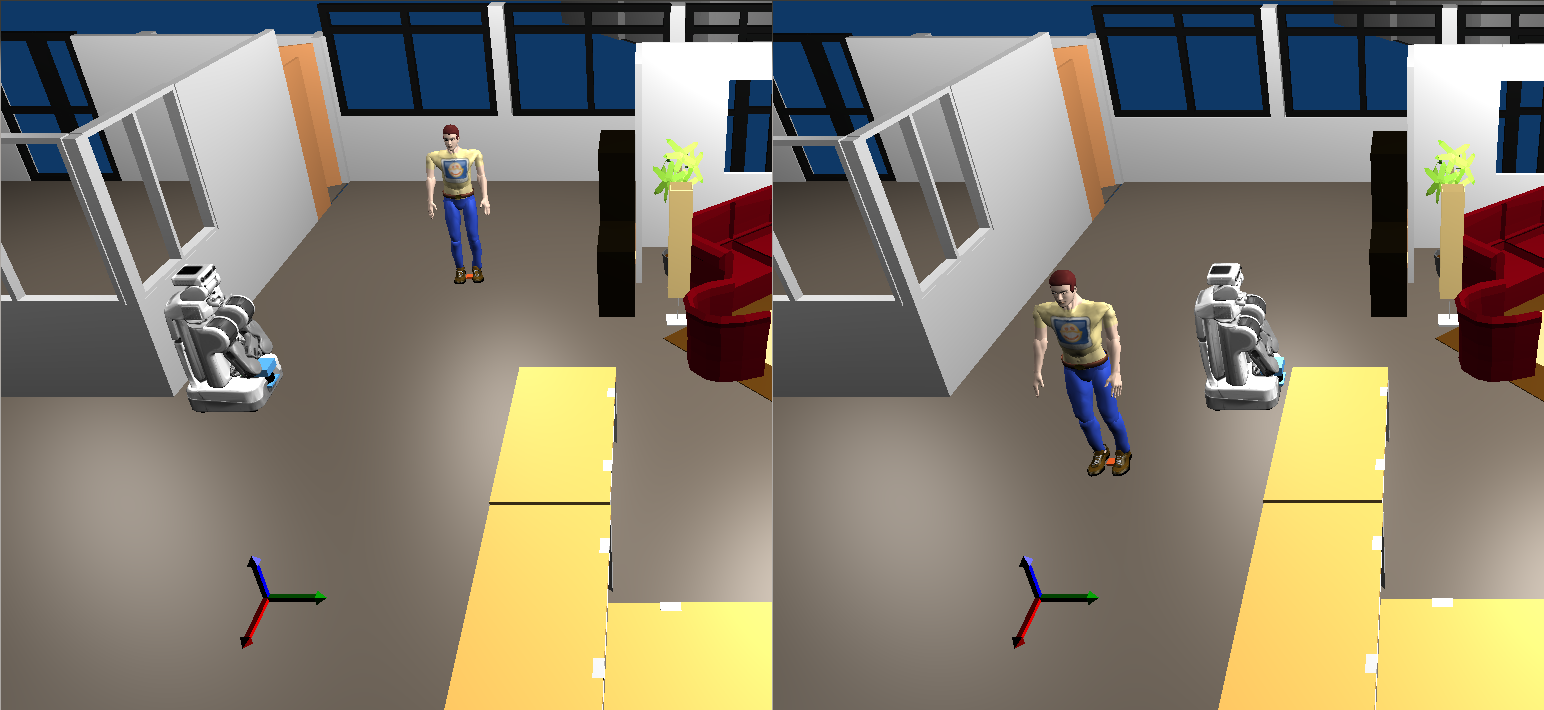
\includegraphics[width=0.9\linewidth]{morsehanp.png}
      \caption{Navigation test with MORSE}
      \label{fig|hanp}
\end{figure}

%   3- what is good and could be useful to other researcher
\emph{Usefulness:} Full support of the PR2 robot model among others,
availability of a human model, and a convenient way of setting up experiment
environment using Blender software were the most prominent features for choosing
Morse as the simulation environment for these experiments. Since Morse already
provides ROS bindings for the PR2 robot and human pose, it requires minimal
effort to switch between real-world and simulated environments. The real-world
experiment results were later published in \cite{ThibaultKruse2014}.

% future use of morse
As a consortium member in the EU project
SPENCER\footnote{\url{http://www.spencer.eu}}, we are interested in developing
novel algorithms for robot navigation in large populated environments,
e.g. airports. In the future we plan to use Morse to simulate such large
environment with multiple human models. This will certainly push the limits of
simulation for HRI and hopefully provide new benchmark for Morse.

%   4- what is missing both at the technical level (things that could be added
%      to MORSE) and at a more fundamental level (things where simulation do
%      not fit)
% fundamental: implementing human behaviors? e.g. crowd simulation
\emph{Missing features:} All DOFs of the human posture in MORSE already has an
interface support for pocolibs and yarp middleware. It would be a valuable
addition to MORSE to add a ROS interface for the same, and publish all these
DOFs as coordinate frames using the typical `tf' package. Moreover, an easier
way to attach camera to the human eyes would be appreciated. For HRI experiments
this will give a human perspective on the robot actions and its effects on the
environment.


\subsection{Data Acquisition through Automatic Scene Generation}
\label{sc:generation}

\emph{Use-Case:} Autonomous mobile robots that are to help and assist people in
care homes, households, and at other workplaces have to understand how human
activities affect the dynamics of objects in the environment. That is, robots
need to know, when, where and how people manipulate objects and how they
arrange and structure them in space. In the context of the STRANDS
project\footnote{\url{http://www.strands-project.eu}} we aim for robots that
understand the long-term, spatio-temporal relationships of objects and
activities of people. In the scenario described in this paper, we looked in
particular at learning qualitative spatial relations of objects on office
desks. As an accurate classification and pose estimation of objects on
real-world office desks is still a challenging and difficult task for current
robot perception systems we acquired a data set of object arrangements using
the MORSE simulator. For this, we first bootstrapped an object statistics from
manually labeled images of real office desks, and secondly, automatically
generated a set of physically possible desktop scenes (see
Figure~\ref{fig:simulated-desktop-scenes}, \cite{kunze14bootstrapping}). Based
on the generated data we learned relational models of object arrangements on
desks. The learnt models enabled a robot to predict the position of an object
given a landmark. We employed these models to effectively guide a simulated and
a real robot in object search tasks and evaluated its performance
\cite{kunze14indirect}.

\emph{Usefulness:} Firstly, the automatic scene generation and annotation of
object arrangements in simulation is useful for the acquisition of large
amounts of data over short periods of time. The generated data enabled us to
design, implement and to evaluate our methods for predicting object locations
before having a real-world data set in place. Secondly, the generation of
object arrangements can increase the variability of scenes in Human-Robot
experiments in general. Given the dynamics of objects in the real world it is
important not to oversimplify Human-Robot experiments in simulated environments
but make them as realistic as possible (in a controlled way). Finally, in
future work, we plan to use the generated desktop scenes in web-applications to
crowdsource Natural Language descriptions of object arrangements and commands
for robots from Internet users.

\emph{Missing features:} The default installation of MORSE already includes a
fair set of pre-modeled objects. However, these objects are spread over
different environments and lack a coherent definition with respect to their
reference frame, bounding box, and/or scale. A desirable feature would be that
objects are kept in a global or some domain specific object databases and that
they are modeled in a consistent way. This would ease the usage of different
types of objects and thereby allow users and researchers to focus on their
goals. Also the addition and/or removal of objects at run-time would be a nice
feature as a running MORSE instance could be used more flexible, for example,
as a robot's belief state.

\begin{figure}[tb]
  \centering
  \includegraphics[width=.9\columnwidth]{figs/scenes.png}
  \caption{Automatically generated scenes of office desks.}
  \label{fig:simulated-desktop-scenes}
\end{figure}


\subsection{Automated Execution of Prototype HRI Experiments}
\label{sc:ci}

% 1 - why simulation is useful/needed for your use-case
\emph{Use-Case:} In Human-Robot Interaction studies, robots often indicate
behavioral variability that may influence the experiment's final outcome.
However, manual testing on physical systems is usually the only way to prevent
this, but remains labour-intensive. To tackle this issue, we introduced
\emph{early automated prototype testing} \cite{2645922} that consists of: a
simulation environment, a software framework for automated bootstrapping of
prototype systems, execution verification of system components, automated result
assessment of experiments \cite{2563606} and a Continuous Integration (CI)
\cite{duvall2007continuous} server to centralize experiment execution. In our
setup we bootstrap and execute a simulated prototype system on a CI server and
assess the results in each run. In this particular scenario, a robot must report
the location of a virtual human in a domestic environment. Both, the robot and
the human, are moving about in the scene and meet in front of a table
(Figure~\ref{fig|proto}).

\begin{figure}[H]
      \centering
      \includegraphics[width=0.9\linewidth]{proto-setup.png}
      \caption{Prototype HRI Simulation.}
      \label{fig|proto}
\end{figure}

The goal of this simulation setup is to incrementally decrease the level of
abstraction until a satisfactory/sufficient degree of ``realism'', to make an
assumption about real world behavior, is reached --- in an integrated and
continuous approach. In order to realise this goal, we make use of two essential
MORSE features: a) the human avatar that can be steered (set waypoints)
interactively via middleware and b) a semantic camera
\footnote{\url{openrobots.org/morse/doc/stable/user/sensors/semantic_camera.html}}
that extracts the location of a specific entity in the simulation environment.
The semantic camera is attached to the robot. If the human enters the robot's
field of view, the location is reported and sent via middleware. After each CI
run, the recorded movement trajectory of the human avatar is assessed (plotted)
and archived. 
% 2 - is it satisfactory or not
We have explicitly chosen to simplify the extraction of the
human's location to acquire a ground truth in the first iterations of the
simulation. Based on the ground truth, we are able to exchange diverse
components, i.e., the semantic camera with a simulated laser scanner
\footnote{\url{openrobots.org/morse/doc/stable/user/sensors/laserscanner.html}},
to build a person hypothesis for instance, thus gradually develop, assess and
implement more complex scenarios. 

%3 - usefulness
\emph{Usefulness:} First of all, the interactive (remotely controllable) human avatar 
is useful to include a dynamic, yet not too realistic, human component in this 
setup, which currently is a rare feature in the world of simulators. Secondly, 
the level of abstraction of different sensors, i.e., semantic camera versus virtual 
laser scanner enables us to gradually raise the level of complexity/realism and 
test different algorithms based on abstract and almost realistic sensor inputs. 
Lastly, the chance to deploy MORSE in a Continuous Integration environment, i.e., 
automatically run ``builder scripts'' \footnote{\url{http://www.openrobots.org/morse/doc/latest/dev/builder.html}}
generates an additional benefit.
 
%4 - missing features
\emph{Missing features:} To be even more useful, simulators and thus MORSE, must
feature a realistic ``walking cycle'' for human components. This is especially
important if laser scans are used to build a person hypothesis. Additionally, the
human avatar should feature (remotely) triggered ``actions'', e.g., grasping a 
predefined object, sit down on a chair/sofa or open a door. Lastly, audio support, 
i.e., Text-to-Speech output for the human component would significantly increase
the usability to assess algorithms which rely on multimodal inputs.  

\section{Discussion: Which Place for HRI Simulation?}

As researchers in HRI, we believe that simulation holds a rightful place, both as
an efficient engineering support tool, and as a novel source of realistic yet
repeatable (hence comparable) human inputs for our systems.

The five scenarii that are presented here cover as such a range of use-cases.
Using a simulator to provide a reference environment with repeatable conditions
(as in scenarii~\ref{sc:assessment}, \ref{sc:expectations} and
\ref{sc:navigation}) is the expected role of a simulator. MORSE simply provides
additional tools to represent and control humans, either in perfectly repeatable
ways (by pre-programming the human behaviour) or in less repeatable but also
more realistic ways (in the ``first-person shooter'' mode).

But other use-cases emerge: data synthesis and acquisition for complex and
dynamic human environments (scenario~\ref{sc:generation}), collaboration between
universities over human-robot interaction situations
(scenario~\ref{sc:assessment}), and automatic testing of robotic softwares that
involve humans (scenario~\ref{sc:ci}).

These diverse use-cases support the idea that simulation is not only actually
useful as a support tool for development of human-robot applications, but also
\emph{enables} new development workflows in HRI. \emph{Continuous Integration}
illustrates this point: while HRI experiments are considered as notoriously
difficult to deploy, test and repeat, we show here that our recent progresses in
software engineering enable automatic testing of more and more complex scenarii,
including long-term interaction.

%I think we are "not yet there" on any of these items, but that's where
%we aim to go, and this could hopefully sketch/define a new toolset for
%future HRI research.
%
%- (automatic) testing of human-robot *interaction*, which is notoriously
%difficult (in particular because human behaviours are mostly non
%repeatable) (and until now, no simple solution exist for that)


\paragraph*{The next steps}

Several noteworthy developments related to HRI are currently shaping up in the
MORSE community. We outline below some of them, that suggest new applications we
believe relevant to HRI research.

A first line of investigation relates to the procedural generation of a variety
of realistic human models. {\sc MakeHuman} is such an open-source tool that
generates anatomically, kinetically and visually realistic human models
(Figure~\ref{fig:makehuman}. This software has a tight integration with Blender,
and MORSE is soon to provide as well seamless integration with {\sc MakeHuman}
models. This would provide a wide range of characters to feed the simulations,
and extend testing environments with gender/size/age/skin color variances.  For
this feature to reach its full potential, {\sc MakeHuman} should however be
extended to support programmatic generation of models, since the graphical user
interface is currently required.

\begin{figure}[tb]
  \centering
  \includegraphics[width=.9\columnwidth]{figs/makehuman.png}
  \caption{Procedural generation of human models with {\sc MakeHuman}.}
  \label{fig:makehuman}
\end{figure}

Besides being able to control a human avatar in simulation programmatically and
deterministically, the possibility to automatically generate believable and
realistic crowd behaviours is being explored. In this context, the objective is
to adopt technologies successfully deployed computer games in MORSE to generate
trajectories that control the MORSE avatars.  Based on the idea of \emph{social
forces}~\cite{helbing2001}, the work of~\cite{Szymanezyk2012crowd} is to be
adopted to provide believable and realistic movement of several humans within
MORSE. The approach is based on a grid-based representation that computes forces
for individual agents which are computed from combining information from other
agents (\eg taking social distances and group forming into account), from the
environment (\eg implementing obstacle avoidance), and from a pre-defined set of
goals individually defined for each agent. The resulting velocity vector for
each agent can be directly interfaced with several instances of MORSE avatar to
generate natural movement trajectories. This implementation can provide a more
realistic and dynamic environment to study human-robot spatial interaction and
to provide a testbed for human-aware motion planning, to give two exemplary use
cases.

Another line of investigation looks at embedding the human into the robotic
simulation. The purpose of such efforts is to provide a life-like immersive
simulation environment that would allow at the same time ecologically valid
human behaviours and repeatable, lightweight interaction settings.
In~\cite{lemaignan2012morse}, we presented how a human agent could interact with
a virtual robot through a gestual interface based on a Kinect. While arm
movements and small displacement (in a 2-3m\textsuperscript{2} zone) could be fairly
accurately transposed from the physical world to the simulation, the overall
interaction was not immersive (no head tracking, limited, non-dynamic field of
view on a TV screen, no sound). Two distinct projects are currently looking into
extending this line of research, one (at Bielefield University) aiming at
integrating emerging Virtual Reality devices (like Occulus Rift) with MORSE, the
other one (MarDI project) developing a virtual reality cave, that include 360°
projections and spatialized sound.

Also often suggested, the \emph{on-line} deployment of HRI simulations could
efficiently support large scale HRI studies. The simulator and specific
interaction scenarii would be embedded in a dedicated webpage and users would
control a human avatar from their webbrowsers. This would potentially enable
collection of large behavioural datasets. While MORSE development in that
direction has yet to start, it can be noted that the Gazebo simulator already
features a limited WebGL client, that act as a proof-of-concept.

\paragraph*{To conclude}

These examples and ideas hopefully give a picture of the lively landscape of the
``Simulation for HRI'' community, that has built itself around the MORSE
simulator.

In the introduction, we mentioned how simulation in HRI had to address in
parallel constraints stemming from \emph{robotic simulation} and \emph{virtual
agent simulation}, while remaining a lightweight, easy-to-use tool. We are
certainly not yet there, much remains to be imagined, refined and achieved. And
yet MORSE is already deployed in several institutions as a platform that
efficiently supports research in human-robot interaction. As an open-source
project, we strive for new use-cases and ideas, and warmly welcome researchers
that would like to join the effort.



%\section*{Acknowledgment}
%TODO

\bibliographystyle{abbrv}
\bibliography{main}

\end{document}
